%%%%%%%%%%%%%%%%%%%%%%%%%%%%%%%%%%%%%%%%%%%%%%%%%%%%%%%%%%%%%%%
%%%  NEF = NESS of a driven Ring, flutuations 
%%%%%%%%%%%%%%%%%%%%%%%%%%%%%%%%%%%%%%%%%%%%%%%%%%%%%%%%%%%%%%%

\documentclass[aps,prl,floats,floatfix,twocolumn]{revtex4}

% special 
\usepackage{ifthen}
\usepackage{ifpdf}
\usepackage{color}

\ifpdf
\usepackage{graphicx}
\usepackage{epstopdf}
\else
\usepackage{graphicx}
\usepackage{epsfig}
\fi
\graphicspath{{./Figs/}{./}}

% fonts
\usepackage{latexsym}
\usepackage{amsmath}
\usepackage{amssymb}
\usepackage{bm}
\usepackage{wasysym}

\usepackage{hyperref}

%%%%%%%%%%%%%%%%%%%%%%%%%%%%%%%%%%%%%%%%%%%%%%%%%%%%%%%%%%%%%%%%

% NEW 
\newcommand{\abs}[1]{\left|#1\right|}
\newcommand{\Prob}{\mbox{Prob}\,}
\newcommand{\erf}{\mbox{erf}\,}
\newcommand{\df}{{\rm d}}

% math symbols I
\newcommand{\sinc}{\mbox{sinc}}
\newcommand{\const}{\mbox{const}}
\newcommand{\trc}{\mbox{trace}}
\newcommand{\intt}{\int\!\!\!\!\int }
\newcommand{\ointt}{\int\!\!\!\!\int\!\!\!\!\!\circ\ }
\newcommand{\ar}{\mathsf r}
\newcommand{\im}{\mbox{Im}}
\newcommand{\re}{\mbox{Re}}

% math symbols II
\newcommand{\eexp}{\mbox{e}^}
\newcommand{\bra}{\left\langle}
\newcommand{\ket}{\right\rangle}

% Mass symbol
\newcommand{\mass}{\mathsf{m}} 
\newcommand{\Mass}{\mathsf{M}} 

% more math commands
\newcommand{\tbox}[1]{\mbox{\tiny #1}}
\newcommand{\bmsf}[1]{\bm{\mathsf{#1}}} 
%\newcommand{\amatrix}[1]{\matrix{#1}} 
\newcommand{\amatrix}[1]{\begin{matrix} #1 \end{matrix}} 
\newcommand{\pd}[2]{\frac{\partial #1}{\partial #2}}

% equations
\newcommand{\mylabel}[1]{\label{#1}} 
%\newcommand{\mylabel}[1]{\textcolor{blue}{[#1]}\label{#1}} 
\newcommand{\beq}{\begin{eqnarray}}
\newcommand{\eeq}{\end{eqnarray}} 
\newcommand{\be}[1]{\begin{eqnarray}\ifthenelse{#1=-1}
{\nonumber}{\ifthenelse{#1=0}{}{\mylabel{e#1}}}}
\newcommand{\ee}{\end{eqnarray}} 

% arrangement
\newcommand{\drawline}{\begin{picture}(500,1)\line(1,0){500}\end{picture}}
\newcommand{\bitem}{$\bullet$ \ \ \ }
\newcommand{\Cn}[1]{\begin{center} #1 \end{center}}
\newcommand{\mpg}[2][1.0\hsize]{\begin{minipage}[b]{#1}{#2}\end{minipage}}
\newcommand{\mpgt}[2][1.0\hsize]{\begin{minipage}[t]{#1}{#2}\end{minipage}}
\newcommand{\sect}[1]{{\bf #1.-- }}


% more
%\newcommand{\Eq}[1]{Eq.\!\!~(\ref{#1})}
%\newcommand{\Fig}[1]{Fig.\!\!~\ref{#1}}  
\newcommand{\Eq}[1]{\textcolor{blue}{Eq.\!\!~(\ref{#1})}} 
\newcommand{\Fig}[1]{\textcolor{blue}{Fig.}\!\!~\ref{#1}} 
\newcommand{\hide}[1]{}
%\newcommand{\hide}[1]{\textcolor{red}{[hidden text]}} %{}
\newcommand{\rmrk}[1]{\textcolor{red}{#1}}
%\newcommand{\Rmrk}[1]{\textcolor{blue}{\LARGE\bf #1}}

%\renewcommand{\includegraphics}[2][]{\ \\ \ FIGURE: \ \\ \ }
\renewcommand{\cite}[1]{\textcolor{blue}{[\onlinecite{#1}}]} %{[\onlinecite{#1}]} 


%\def\circbul{{\bigcirc \mkern-8mu _{\bullet} \mkern-8mu}} 
%\newcommand{\overline}[1]{\overline{#1}}

%%%%%%%%%%%%%%%%%%%%%%%%%%%%%%%%%%%%%%%%%%%%%%%%%%%%%%%%%%%%%%%%%%%%%%%%%%%%%%%%%%%%%%%%%%
%%%%%%%%%%%%%%%%%%%%%%%%%%%%%%%%%%%%%%%%%%%%%%%%%%%%%%%%%%%%%%%%%%%%%%%%%%%%%%%%%%%%%%%%%%
 
\begin{document}

\title{Non-equilibrium steady state and induced currents of a mesoscopically-glassy system:\\
interplay of resistor-network theory and Sinai physics}

\author{Daniel Hurowitz$^1$, Saar Rahav$^2$, Doron Cohen$^1$}

\affiliation{
\mbox{$^1$Department of Physics, Ben-Gurion University of the Negev, Beer-Sheva, Israel} \\
\mbox{$^1$Schulich Faculty of Chemistry, Technion - Israel Institute of Technology, Haifa 32000, Israel}
}

\begin{abstract}
We introduce an explicit solution for the non-equilibrium steady state (NESS) 
of a ring that is coupled to a thermal bath, and is driven by an external 
hot source with log-wide distribution of couplings. 
Having time scales that stretch over several decades is similar to glassy systems.
Consequently there is a wide range of driving intensities where the NESS 
is like that of a random walker in a biased Brownian landscape. 
We investigate the resulting statistics of the induced current~$I$. 
For a single ring we discuss how $\text{sign}(I)$ fluctuates as the intensity 
of the driving is increased, while for an ensemble of rings we highlight 
the fingerprints of Sinai physics on the $\text{abs}(I)$ distribution.   
\end{abstract}

\maketitle


%%%%%%%%%%%%%%%%%%%%%%%%%%%%%%%%%%%%%%%%%%%%%%%%%%%%%%%%%%%%%%%%%%%%%%%%%

The transport in a chain due to random non-symmetric transition probabilities
is a fundamental problem in statistical mechanics \cite{derrida,d1,d2,d3,d4,sinai,sinai2}.
%
This type of dynamics is of great relevance for surface diffusion \cite{surface}, 
thermal ratchets~\cite{brownian1,brownian2,brownian3,ratchets}  
and was used to model diverse biological systems, 
such as molecular motors, enzymes, and unidirectional motion 
of proteins along filaments \cite{motors1,brownian4,motors2,motors3}.
Of particular interest are applications that concern the conduction 
of DNA segments \cite{DNA1,DNA3}, and thin glassy electrolytes under high voltages 
\cite{Wichmann,Roling1,Roling2,Roling3,Nitzan}.

Mathematically one can visualize the dynamics 
as a {\em a random-walk in a random environment}: 
a particle that makes incoherent jumps between ``sites" of a network.
In an unbounded quasi-one-dimensional network we might have either diffusion 
or sub-diffusive Sinai spreading \cite{sinai}, 
depending on whether the transitions rates 
form a symmetric matrix or not. In contrast, when the system is bounded 
(and without disjoint components) 
it eventually reaches a well-defined steady state. 
This would be an equilibrium {\em canonical} (Boltzmann) state if the transition rates 
were detailed-balanced, else it is termed non-equilibrium steady state (NESS). 

\rmrk{We consider the NESS of a mesoscopically glassy system.
{\em Our working hypothesis is that glassiness might lead to a novel NESS
with fingerprints of Sinai physics.}}
%
By ``glassiness" we mean that the rates that are induced by a bath, 
or by an external source, have a log-wide distribution,
hence \rmrk{many time scales are involved} \cite{Rit1} as in spin-glass models \cite{Rit2}.  
%
\rmrk{Having a log-wide distribution of time scales is typical 
for hopping in a random energy landscape, 
where the rates depend exponentially on the barrier heights.
It also arises in driven quasi-integrable systems, 
where due to approximate selection-rules there is a ``sparse" fraction 
of large coupling-elements, while the majority become very small \cite{slk}. }

\rmrk{
We consider a geometrically closed mesoscopic system 
that has a non-trivial topology. The system is immersed in 
a finite temperature ``cold" bath, and additionally 
it is coupled to a driving source. 
The latter can be regarded as a ``hot bath" of infinite temperature. 
Consequently detailed-balance is spoiled, 
and after a transient a NESS is reached. 
%
Specifically we consider the simplest possible model: 
a mesoscopic ring that is made up of~$N$ sites. 
See \cite{SM} for a graphical illustration.
%
Due to the lack of detailed-balance a circulating current is induced.
We shall see that the value of the current depends in a non-linear way 
on the intensity of the driving source. Our interest 
is in the statistical aspects of this dependence.        
}


\rmrk{The emergence of Sinai physics in a system that is described 
by a rate equation with asymmetric transition probabilities is 
naturally expected, but not self-evident \cite{Rit3}.
An experimental observation of Sinai diffusion regarding the unzipping 
transition of DNA molecules has been reported \cite{Nelson},
and other applications have been considered \cite{domainwalls,sandpiles}.
%
The non-linear current depedence of a mesoscopic rings has 
been theoretically studied in the past \cite{Wichmann,Nitzan}, 
with references to experiments \cite{Roling1,Roling2,Roling3}, 
but the statistical aspects, and the possible relevance 
of Sinai physics, have not been considered.} 
%
In previous publications, we have pointed out that due to ``glassiness" 
Sinai physics becomes a relevant ingredient in the analysis of energy 
absorption \cite{kbb} and transport \cite{ner} in such a ring system.



%%%%%%%%%%%%%%%%%%%%%%%%%%%
\sect{Scope}
%
Below we introduce an explicit NESS solution for a minimal model that 
has all the essential ingredients of the problem, involving transitions between sites on a ring 
and a log-wide distribution of couplings to an external driving source. 
The induced steady state current~$I$ is the central quantity used to characterize 
the NESS in actual experiments. The purpose of the present study is to investigate 
its statistics. Specifically, for a single ring we discuss how $\text{sign}(I)$ fluctuates    
as the intensity of the driving is increased, while for an ensemble 
of rings we highlight the fingerprints of Sinai physics on the $\text{abs}(I)$ distribution.  
%
\rmrk{Our model construction is physically motivated and significantly differs 
from the standard setup of e.g.\cite{sinai2}, see \cite{rm}.}


%%%%%%%%%%%%%%%%%%%%%%%%%%%%%%%%%%%%%%%%%%%%%%%%%%%%%%%%%%%%%%%%%%%%%%%%%%%%%%%%%
%%%%%%%%%%%%%%%%%%%%%%%%%%%%%%%%%%%%%%%%%%%%%%%%%%%%%%%%%%%%%%%%%%%%%%%%%%%%%%%%%
\sect{The model}
%
%
Consider a ring that consists of sites labeled by~$n$ 
with positions ${x=n}$ that are defined modulo~$N$. 
The bonds are labeled as ${\overrightarrow{n}\equiv(n{-}1 \leadsto n)}$.
The inverse bond is $\overleftarrow{n}$, and if direction does 
not matter we label both by $\bar{n}$. The position of the $n$th bond 
is defined as $x_n \equiv n{-}(1/2)$. The on-site energies $E_n$ 
are normally distributed over a range $\Delta$,  
and the transitions rates are between nearest-neighboring sites:   
%
\beq
w_{\overrightarrow{n}} \ \ = \ \ w^{\beta}_{\overrightarrow{n}} + \nu g_{\bar{n}}
\eeq 
%
Here $w^{\beta}$ are the rates that are induced by a bath that has 
a finite temperature $T_B$. The $g_{\bar{n}}$ are 
couplings to a driving source that has an intensity~$\nu$. 
These couplings are log-box distributed within ${[g_{\text{min}},g_{\text{max}}]}$.
This means that $\ln(g_{\bar{n}})$ are distributed uniformly 
over a range ${\sigma=\ln(g_{\text{max}}/g_{\text{min}})}$. 
%
%
%
%
The bath transition rates satisfy detailed-balance, 
namely $w^{\beta}_{\overrightarrow{n}}/w^{\beta}_{\overleftarrow{n}} = \exp[-(E_{n}{-}E_{n{-}1})/T_B]$.
The driving spoils the detailed-balance. We define the resulted 
stochastic field as follows:
%
\be{100}
\mathcal{E}(x_n) \ \ \equiv \ \ \ln \left[\frac{w_{\overrightarrow{n}}}{w_{\overleftarrow{n}}}\right] 
\ \approx \ - \left[ \frac{1}{1+g_{\bar{n}}\nu} \right] \frac{E_n{-}E_{n{-}1}}{T_B}
\ee
%
where the last equality assumes ${\Delta \ll T_B}$ (see \cite{SM})
and without loss of generality the $g_{\bar{n}}$ have been re-scaled 
such that all the bath-induced transitions have 
the same average transition rate ${\bar{w}^{\beta}=1}$. 

%%%%%%%%%%%%%%%%%%%%%%%%%%%
\sect{The direction of the current}
%
%
$\text{sign}(I)$ is determined by the 
stochastic motive force (SMF), also known as the affinity, 
or as the entropy production \cite{eprd1,eprd2,eprd3,eprd4}:
%
\be{101}
\mathcal{E}_{\circlearrowleft} 
\ \ \equiv \ \ \ln \left[\frac{ \prod_n w_{\overrightarrow{n}}}{ \prod_n w_{\overleftarrow{n}}}\right] 
\ \ = \ \ \oint \mathcal{E}(x) \, dx 
\ee
%
\rmrk{In the second equality we formally regard $x$ as a continuous variable.
This will make the later mathematics more transparent.}  
%
Using \Eq{e100} one observes that for ${\nu \ll g_{\text{max}}^{-1}}$ 
the SMF is linear ${\mathcal{E}_{\circlearrowleft}\propto \nu}$,  
while for ${\nu \gg g_{\text{min}}^{-1}}$ it vanishes ${\mathcal{E}_{\circlearrowleft}\propto 1/\nu}$.
In the intermediate regime, which we call below {\em the Sinai regime},  
the SMF changes sign several times, see \Fig{f2}. 
Using the notations
%
\be{1021}
\tau \ \ \equiv \ \ \frac{1}{\sigma}\ln(g_{\text{max}}\nu)
\eeq
% 
and $\tau_n = (1/\sigma)\ln(g_{\text{max}}/g_{\bar{n}})$,  
the expression for the SMF takes the following form:
%
\be{102}
\mathcal{E}_{\circlearrowleft}(\tau) = -\sum_{n=1}^N f_{\sigma}(\tau-\tau_n) \frac{E_n{-}E_{n{-}1}}{T_B}
\eeq 
%
where $f_{\sigma}(t)\equiv [1+\eexp{\sigma t}]^{-1}$ is like a step function.
If $f(t)$ were a sharp step function it would follow
that in the Sinai regime $\mathcal{E}_{\circlearrowleft}(\tau)$ 
is formally like a random walk \cite{rw1,feller,dwass}. 
The number of sign reversals equals the number of times 
the random walker crosses the origin. We have here a coarse-grained 
random walk: the $\tau_n$ are distributed uniformly over a range ${[0,1]}$,  
and each step is smoothed by $f_{\sigma}(t)$ such that the 
effective number of coarse-grained steps is $\sigma$.  
Hence we expect the number of sign changes to be not $\sim\sqrt{\pi N}$ 
but $\sim\sqrt{\pi \sigma}$, reflecting the log-width of the distribution.


%%%%%%%%%%%%%%%%%%%%%%%%%%%%%%%%%%%%%%%%%%
\sect{Adding bonds in series}
%
%
The NESS equations are quite simple and can be solved using elementary 
algebra as in \cite{Wichmann,Roling1,Nitzan,ner}, 
or optionally using the network formalism for stochastic systems \cite{net1,net2,net3}.
Below we propose a generalized resistor-network approach 
that allows to obtain a more illuminating version for the NESS, 
that will provide  better insight for the statistical analysis.  
Let us assume that we have a NESS with a current $I$. 
The steady state equations for two adjacent bonds are 
%
\beq
I &=& w_{\overrightarrow{1}} p_{0} - w_{\overleftarrow{1}}p_{1} \\
I &=& w_{\overrightarrow{2}} p_{1} - w_{\overleftarrow{2}}p_{2}
\ee
%
We can combine them into one equation: 
%
\be{8}
I = \overrightarrow{G} p_{0} - \overleftarrow{G} p_{2},  
\ \ \ \ \ 
\overrightarrow{G} \equiv 
\left[ \frac{1}{w_{\overrightarrow{1}}} + 
\frac{1}{w_{\overrightarrow{2}}} 
\left(\frac{w_{\overleftarrow{1}}}{w_{\overrightarrow{1}}}\right) \right]^{-1}
\eeq
%
and similarly for $\overleftarrow{G}$, see \cite{SM}. 
We can repeat this procedure iteratively.  
If we have $N$ bonds in series we get
%
\beq
\overrightarrow{G} \  \ = \ \ \left[ \sum_{m=1}^N \frac{1}{w_{\overrightarrow{m}}} 
\,\exp\left(-\int_0^{m{-}1}\!\!\!\!\!\!\!\mathcal{E}(x)dx \right) \right]^{-1} 
\eeq
%
Coming back to the ring, we can cut it at an arbitrary site~$n$, 
and calculate the associated $G$s. 
It follows that ${I=(\overrightarrow{G}_n- \overleftarrow{G}_n) \, p_{n}}$.
Consequently the NESS is
%
\beq
p_{n} \ \ = \ \ \frac{I}{\overrightarrow{G}_n- \overleftarrow{G}_n} 
\eeq
%
and  $I$ can be regarded as the normalization factor:
%
\be{11}
I \ = \ \left[\sum_{n=1}^N \frac{1}{\overrightarrow{G}_n-\overleftarrow{G}_n}\right]^{-1}
\eeq    
%
In the next paragraph we show how to write these results 
in an explicit way that illuminates the relevant physics. 



%%%%%%%%%%%%%%%%%%%%%%%%%%%%%%%%%%%%%%%%%%
\sect{The NESS formula}
%
%
We define the conductance of a bond as the geometric mean 
of the clockwise and anticlockwise transmission rates: 
%
\beq  
w(x_n) \ \ = \ \ \sqrt{ w_{\overrightarrow{n}} w_{\overleftarrow{n}} }
\eeq
%
Hence $w_{\overrightarrow{n}} = w(x_n) \exp[(1/2)\mathcal{E}(x_n)]$.
Accordingly 
%
%
\be{13}
\overrightarrow{G}_n = \left[ \sum_{m=n+1}^{N+n} \frac{1}{w(x_m)} 
\,\exp\left(-\int_{n}^{x_m} \!\!\!\mathcal{E}(x)dx \right) \right]^{-1} 
\eeq
%
With the implicit understanding that the summation and the integration 
are anticlockwise modulo $N$. With the new notations it is easy to see 
that ${\overleftarrow{G}_n = \exp(-\mathcal{E}_{\circlearrowleft}) \, \overrightarrow{G}_n}$.
We use the notation $G_n$ for the geometric mean. Consequently 
the formula for the current takes the form 
%
\beq
I \ \ = \ \ \left[\sum_{n=1}^N \frac{1}{G_n}\right]^{-1} 2\sinh\left(\frac{\mathcal{E}_{\circlearrowleft}}{2}\right)
\eeq 
%
while $p_n\propto 1/G_n$. Our next task is to find a tractable
expression for the latter. Regarding $x$ as an extended coordinate, 
the potential $V(x)$ that is associated with the field $\mathcal{E}(x)$ 
is a tilted periodic potential. Adding $[\mathcal{E}_{\circlearrowleft}/N] x$
we get a periodic potential $U(x)$, see \Fig{f3}. Accordingly 
%
\beq
\int_{x'}^{x''} \!\!\!\mathcal{E}(x)dx \ = \ U(x'){-}U(x'') + \frac{\mathcal{E}_{\circlearrowleft}}{N}(x''{-}x')
\eeq  
%
With any function $A(x)$ we can associate a smoothed version 
using the following definition  
%
\beq
\sum_{r=1}^N A(x{+}r) \, \eexp{U(x{+}r)- (1/N)\mathcal{E}_{\circlearrowleft}r} \ \equiv \ A_{\varepsilon}(x) \, \eexp{U_{\varepsilon}(x)} 
\eeq
%
In particular the smoothed potential $U_{\varepsilon}(x)$ is defined by this expression with ${A=1}$. 
Note that without loss of generality it is convenient to have 
in mind ${\mathcal{E}_{\circlearrowleft}>0}$. (One can always flip the $x$~direction).  
Note also that the smoothing scale $N/\mathcal{E}_{\circlearrowleft}$ becomes larger for smaller SMF.
With the above definitions we can write the NESS expression as follows:
%
\be{17}
p_n \ \propto \ \left( \frac{1}{w(x_n)} \right)_{\varepsilon} \eexp{-(U(n)-U_{\varepsilon}(n))}
\eeq
%
This expression is physically illuminating, see \Fig{f3}. 
In the limit of zero SMF it coincides, as expected, 
with the canonical (Boltzmann) result. 
For finite SMF the smoothed pre-factor and the smoothed potential
are not merely constants. Accordingly the pre-exponential factor
becomes important and the ``slow" modulation by the Boltzmann factor 
is flattened. If we take the formal limit of infinite SMF 
the Boltzmann factor disappears and we are left with ${p_n \propto 1/w_n}$    
as expected from the continuity equation for a resistor-network. 


%%%%%%%%%%%%%%%%%%%%%%%%%%%%%%%%%%%%%%%%%%
\sect{Statistics of the current}
%
%
From the preceding analysis it should become clear that 
the formula for the current can be written schematically as 
%
\be{112}
I(\nu) \ \ \sim \ \  \frac{1}{N} \, w_{\varepsilon} \, \eexp{-B} \, 2\sinh\left(\frac{\mathcal{E}_{\circlearrowleft}}{2}\right)
\eeq
%
In the absence of a potential landscape ($U(x)=0$) the formula becomes equivalent to Ohm law: 
it is a trivial exercise to derive it if all anticlockwise and clockwise rates are equal 
to the same values $\overrightarrow{w}$ and $\overleftarrow{w}$ respectively, 
hence $w_{\varepsilon}=(\overrightarrow{w} \overleftarrow{w})^{1/2}$, 
and ${\mathcal{E}_{\circlearrowleft}=N\ln(\overrightarrow{w}/\overleftarrow{w})}$.   
In the presence of a potential landscape we have an activation barrier.
Assuming that the current is dominated by the highest peak 
a reasonable estimate would be
%
\be{113}
B = \text{max}\left\{ U(x){-}U_{\varepsilon}(x) \right\} 
\approx& \frac{1}{2} \Big[ \text{max}\{U\} - \text{min}\{U\} \Big] \ \ \ \ 
\eeq 
%
The implication of \Eq{e112} with \Eq{e113} for the {\em statistics} of the current 
is as follows: in the Sinai regime we expect that it will reflect 
the {\em log-wide} distribution of the activation factor, as discussed below, 
while outside of the Sinai regime we expect it to reflect the {\em normal} distributions 
of the total resistance~$w_{\varepsilon}^{-1}$, and of the SMF.  


%%%%%%%%%%%%%%%%%%%%%%%%%%%%%%%%%%%%%%%%%%
\sect{Statistics in the Sinai regime}
%
We now focus on the statistics in the Sinai regime. 
In order to unfold the log-wide statistics it is 
not a correct procedure to plot blindly the distribution 
of $\ln(|I|)$. Rather one should look on the joint 
distribution ${(\mathcal{E}_{\circlearrowleft},I)}$. 
See \Fig{f4}a. The non-trivial statistics is clearly apparent.
In order to describe it analytically we use 
the single-barrier estimate of \Eq{e113}, 
which is tested in \Fig{f4}b. We see that it 
over-estimates the current for small $B$ values 
(flat landscape) as expected, but it can be trusted 
for large $B$ where the Sinai physics becomes relevant. 

In an actual experiment it would be desired to 
extract the statistics from the $I(\nu)$ measurements 
without referring to the SMF. See \Fig{f5}.
Either way this figure confirms that the $I$ statistics
is the same as the barrier ${\exp(-B)}$ statistics. 
We therefore turn to find an explicit expression for the latter. 
%
%
The probability to have a random walk trajectory $X_n=U(x_n)$ within $[X_a,X_b]$ 
equals the survival probability in a diffusion process  
that starts as a delta function at ${X=0}$ 
with absorbing boundary conditions at $X_a$ and $X_b$.   
Integrating over all possible positions of the walls 
such that ${X_b-X_a=2B}$ is like starting with a 
uniform distribution between the walls. From here 
it is straightforward to deduce \cite{SM}
%
\be{20}
\text{Prob}\left\{\text{barrier}<B\right\} \ \sim \ \exp\left[-\frac{1}{2} \left(\frac{\pi \sigma_U}{2B}\right)^2\right] 
\eeq
%
where $\sigma_U^2 = 2D N$ is the variance of the diffusing `points', 
which is determined ny the diffusion coefficient $D\propto \Delta^2$.
Taking into account that for a given~$\nu$ a fraction of the elements
in \Eq{e102} are effectively zero we get 
%
\be{211}
\sigma_U^2 \ \ = \ \ 2 \Delta^2 N  \, \frac{\ln(g_{\text{max}}\nu)}{\sigma}
\eeq  
%  
The validity of the exact version of \Eq{e20}, see \cite{SM}, 
has been verified in \Fig{f4}. No fitting parameters are required. 


%%%%%%%%%%%%%%%%%%%%%%%%%%%%%%%%%%%%%%%%%%
\sect{Summary}
%
%
We have introduced a generalized ``random-resistor-network"
approach for the purpose of obtaining the NESS current
due to nonsymmetric transition rates. Specifically our 
interest was focused on the NESS of a ``glassy" mesoscopic system. 
The NESS expression clearly interpolates the canonical (Boltzmann) result 
that applies in equilibrium, with the resistor-network result, 
that applies at infinite temperature. 
Due to the ``glassiness" the current has novel dependence 
on the driving intensity, and it posseses unique statistical properties 
that reflect the Brownian landscape of the stochastic potential.
This statistics is related to Sinai's random walk problem, 
and would not arise if the couplings to the driving source 
were merely disordered.


%%%%%%%%%%%%%%%%%%%%%%%%%%%%%%%%%%%%%%%%%%%%%%%%%%%%%%%%%%%%%%%%%%%%%%%%%%%%%%%%%%%%
%%%%%%%%%%%%%%%%%%%%%%%%%%%%%%%%%%%%%%%%%%%%%%%%%%%%%%%%%%%%%%%%%%%%%%%%%%%%%%%%%%%%
\clearpage




%%%%%%%%%%%%%%%%%%%%%%%%%%%%%
\begin{figure}
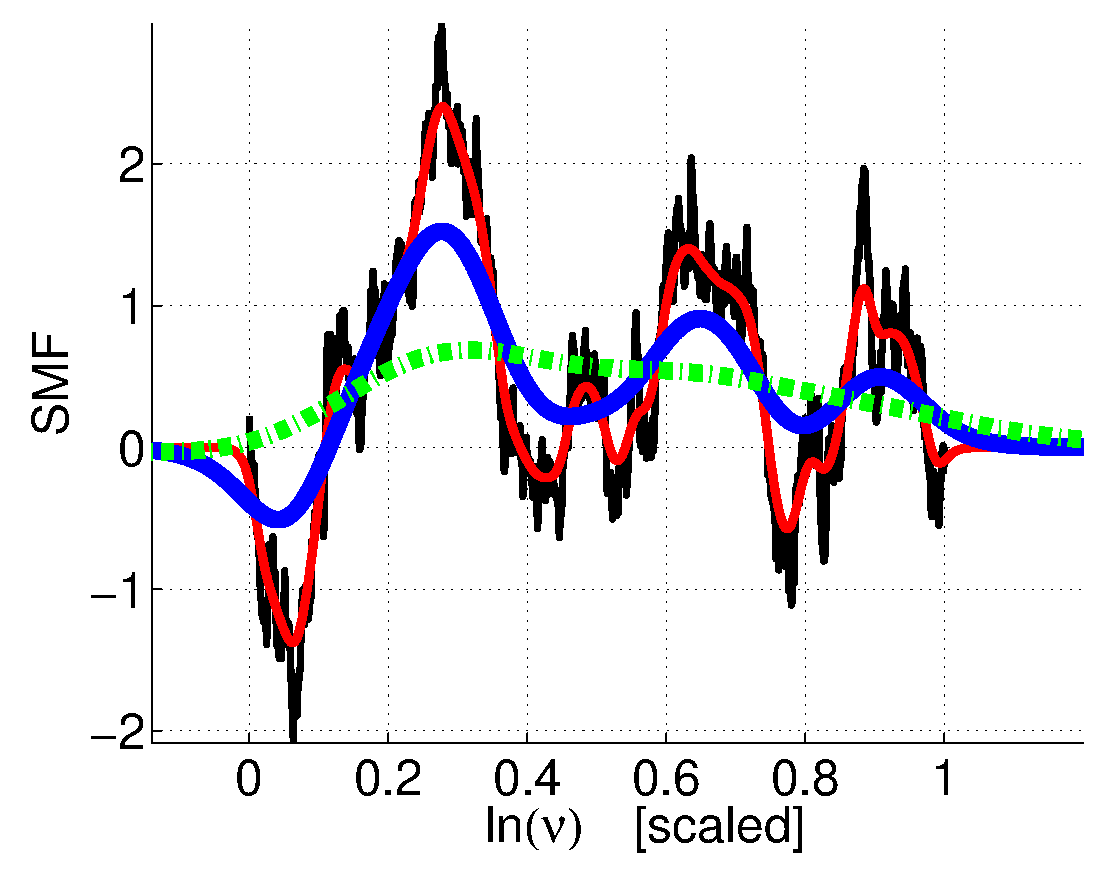
\includegraphics[width=6cm]{SMF_RW.eps}

\vspace*{5mm}

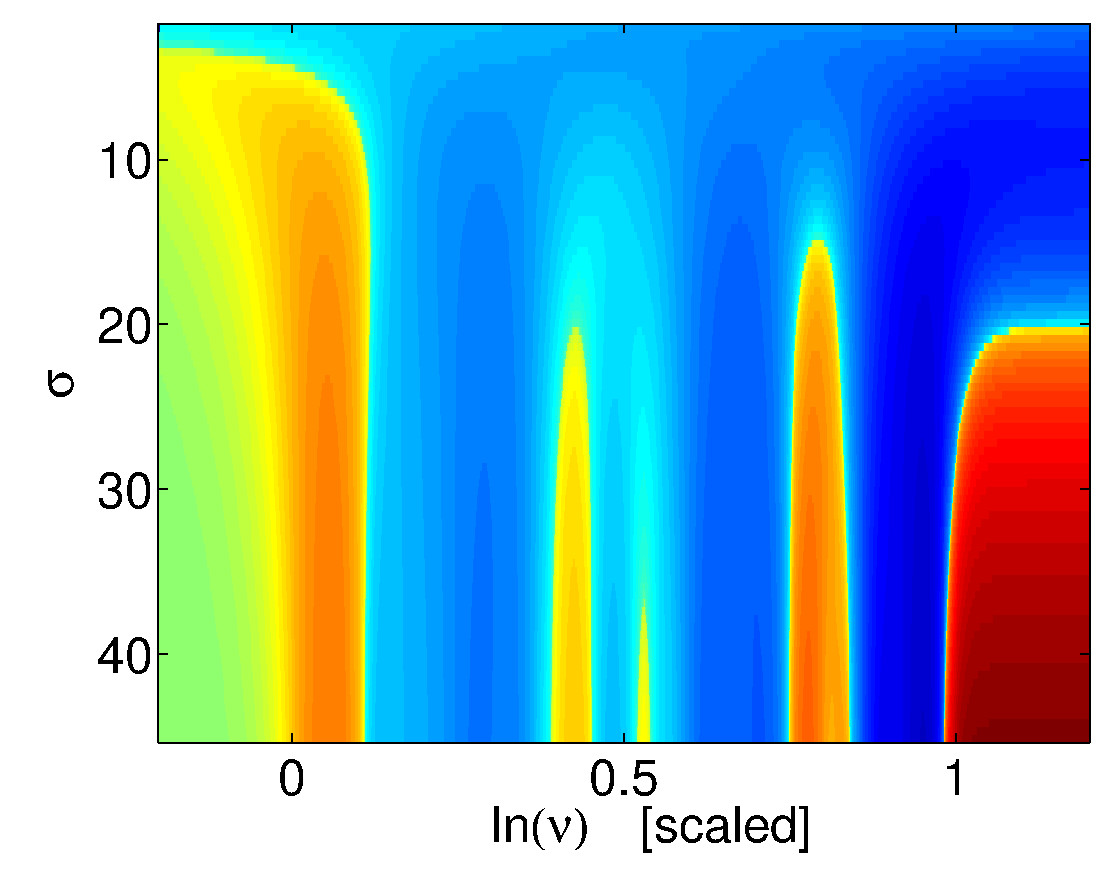
\includegraphics[width=6cm]{I_sig_tau.eps}

\caption{
We consider a ring with ${N=1000}$ sites whose energies 
are normally distributed with dispersion ${\Delta=1}$.
The bath temperature is $T_B=10$. In the upper panel 
the SMF of \Eq{e102} is plotted for $\sigma=\infty$, 
and for $\sigma=50,10,4$. The smaller $\sigma$, 
the smoother $\nu$ dependence. 
This is reflected in the current $I(\nu)$, which is colored 
imaged in the lower panel: each row is for a different $\sigma$,  
\rmrk{blue and red are for positive and negative (clockwise) 
circulating current respectively.}     
In both panels the horizontal axis is 
the scaled driving intensity as defined in \Eq{e1021}.} 
\label{f2}
\end{figure}
%%%%%%%%%%%%%%%%%%%%%%%%%%%%%%



%%%%%%%%%%%%%%%%%%%%%%%%%%%%%%
\begin{figure}
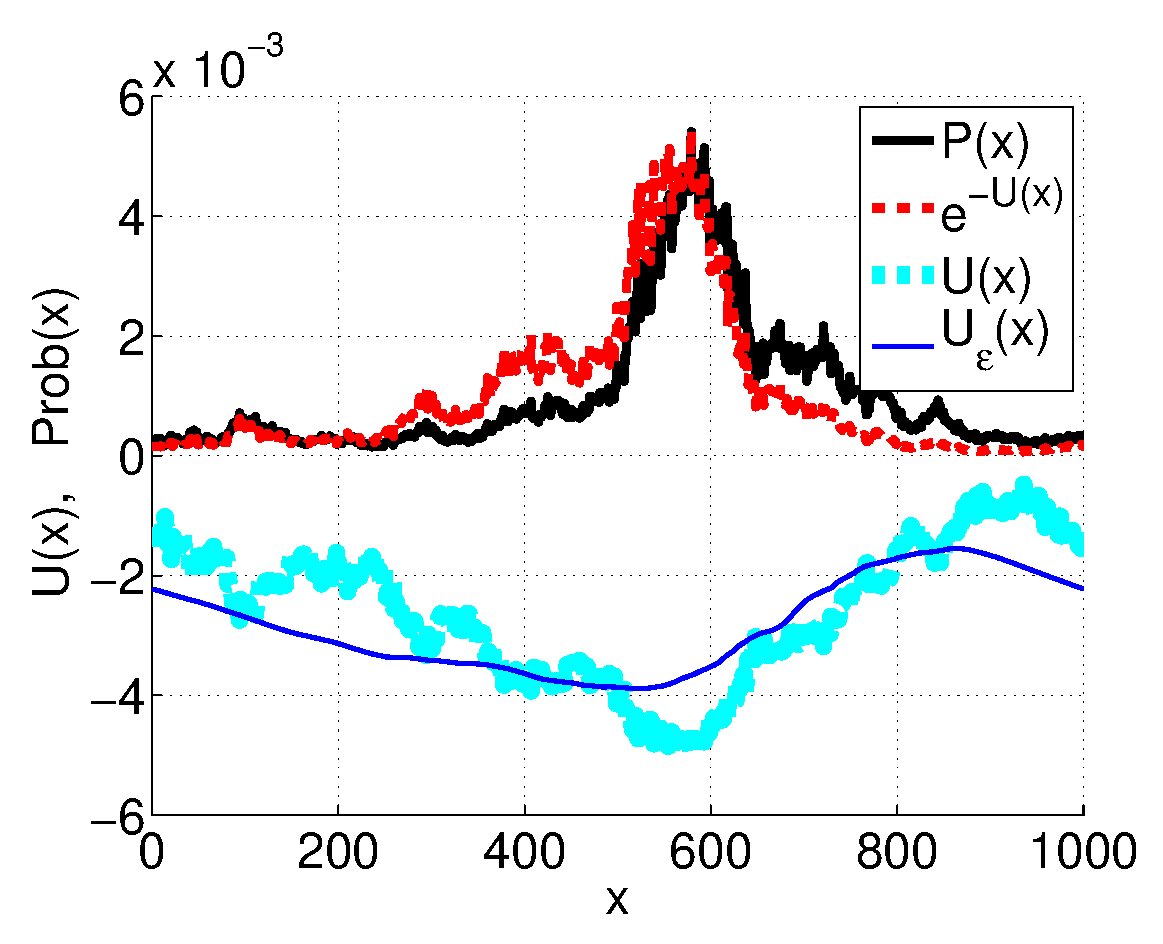
\includegraphics[width=7cm]{PvsV4}

\caption{
The NESS profile of \Eq{e17} (solid black) 
is similar but not identical to the quasi-equilibrium 
distribution (dashed red line). 
Also shown (lower curves) is the potential landscape $U(x)$ 
and its smoothed version $U_{\varepsilon}(x)$. 
The parameters are the same as in \Fig{f2}, 
\rmrk{with $\sigma=10$}, 
and driving intensity that corresponds to $\tau=0.3$.
The bonds were re-arranged to have a larger SMF,
namely $\mathcal{E}_{\circlearrowleft}=7.4$.}

\label{f3}
\end{figure}
%%%%%%%%%%%%%%%%%%%%%%%%%%%%%%



%%%%%%%%%%%%%%%%%%%%%%%%%%%%%%%%%
\begin{figure}

\hspace*{-10mm} (a) \\
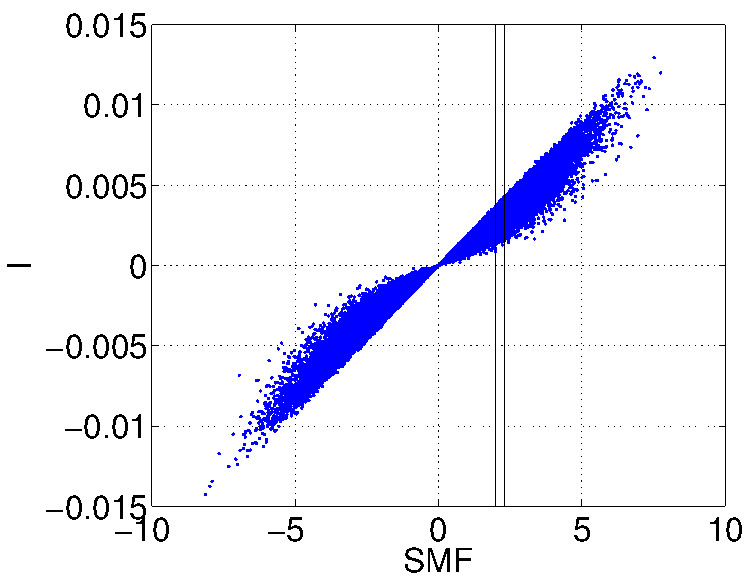
\includegraphics[width=6cm]{IvsSMF2.jpg}

\vspace*{5mm}

\hspace*{-10mm} (b) \\
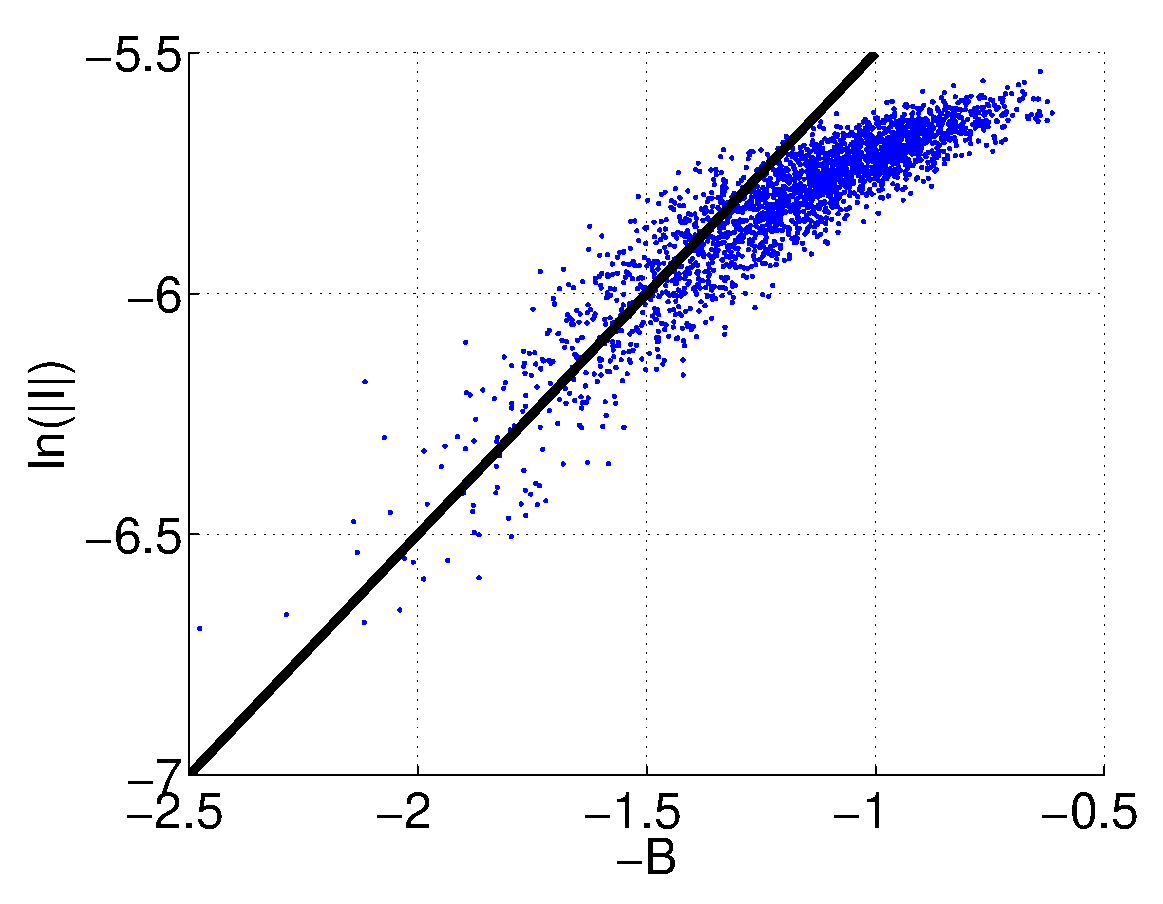
\includegraphics[width=6cm]{BvsLnI.eps}

\caption{(a) Scatter diagram of the current versus the SMF in the Sinai regime.
Note that in the linear regime, see \cite{SM}, it looks like a perfect linear 
correlation with {\em negligible} transverse dispersion.  
(b) The correlation between the current~$I$ and the barrier~$B$,  
within the slice ${\mathcal{E}_{\circlearrowleft} \in [2.0,2.1]}$. 
One deduces that the single-barrier approximation is valid for small currents.}

\label{f4}
\end{figure}
%%%%%%%%%%%%%%%%%%%%%%%%%%%%%%%%%



%%%%%%%%%%%%%%%%%%%%%%%%%%%%%%%%%
\begin{figure}
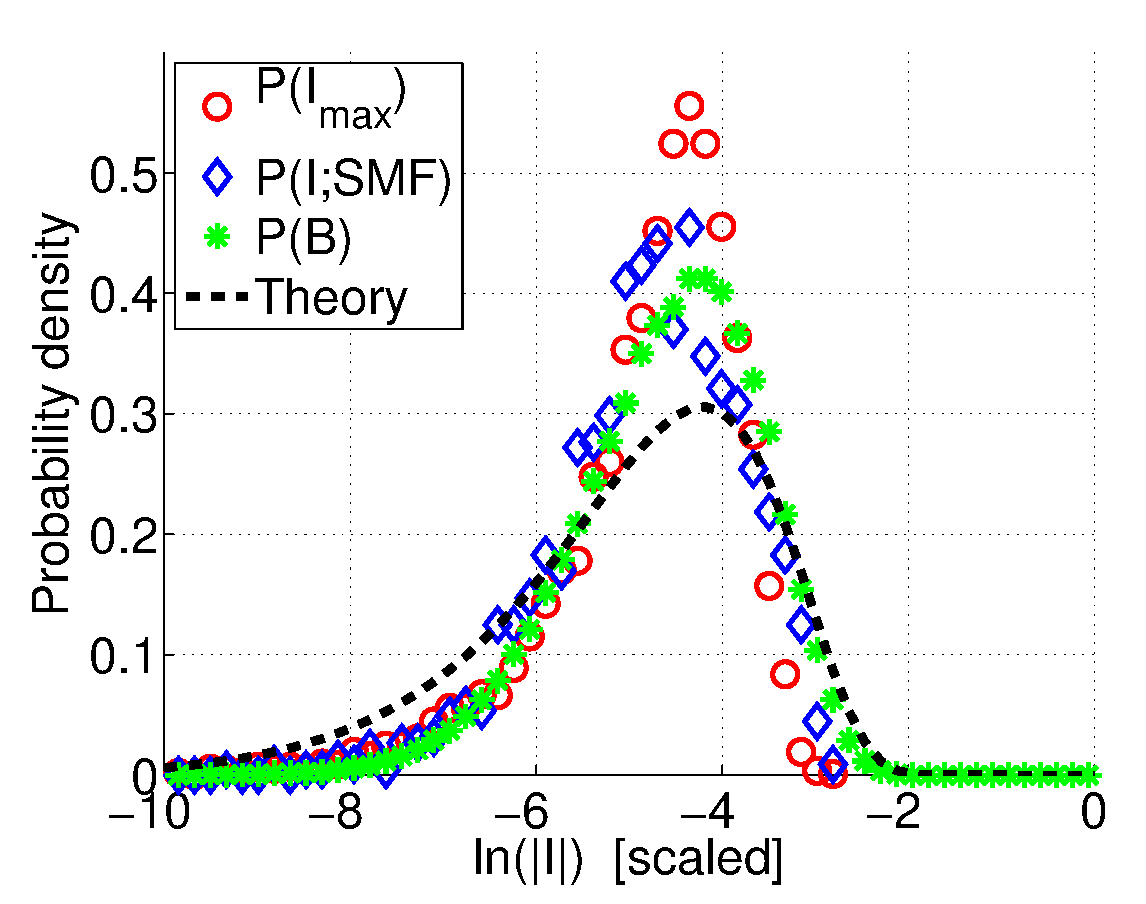
\includegraphics[width=7cm]{PlnI.eps}

\caption{The log-wide distribution $P(I)$ of the current 
in the Sinai regime is revealed provided a proper procedure 
is adopted. For theoretical analysis it is convenient 
to plot an histogram of the~$I$ values for a given SMF:
the blue diamonds refer to the data of \Fig{f4}b.  
%
In an actual experiment it is desired to extract
statistics from $I(\nu)$ measurements without 
referring to the SMF: the red empty circles 
show the statistics of the first maximum of $I(\nu)$.    
%
Both distributions look the same, and reflect 
the barrier statistics (full green circles). 
The line is the exact version \cite{SM} of \Eq{e211}.}

\label{f5}
\end{figure}
%%%%%%%%%%%%%%%%%%%%%%%%%%%%%%%%%


%%%%%%%%%%%%%%%%%%%%%%%%%%%%%%%%%%%%%%%%%%%%%%%%%%%%%%%%%%%%%%%%%%%%%%%%%%%%%%%%%%%%
%%%%%%%%%%%%%%%%%%%%%%%%%%%%%%%%%%%%%%%%%%%%%%%%%%%%%%%%%%%%%%%%%%%%%%%%%%%%%%%%%%%%
\clearpage


%%%%%%%%%%%%%%%%%%%%%%%%%%%%%%%%%%%%%%%%%%%%%%%%%%%%%%%%%%%%%%%%%%%%%%%%%%%%
{\bf Acknowledgments.-- }
%
This research was supported by the Israel Science Foundation (grant No.29/11).
We thank Oleg Krichevsky (BGU) for a useful advice. SR is grateful for support from
the Israel Science Foundation (grant 924/11).


%%%%%%%%%%%%%%%%%%%%%%%%%%%%%%%%%%%%%%%
\begin{thebibliography}{99}

\bibitem{derrida}
B. Derrida, Y. Pomeau, 
% Classical Diffusion on a Random Chain
Phys. Rev. Lett. 48, 627 (1982).

\bibitem{d1}
S. H. Noskowicz, I. Goldhirsch,
% Average versus Typical Mean First-Passage Time in a Random Random Walk
Phys. Rev. Lett. 61, 500 (1988); 
% First-passage-time distribution in a random random walk
Phys. Rev. A 42, 2047 (1990). 

\bibitem{d2}
J. P. Bouchaud, A. Comtet, A. Georges, P. Le Doussal,
% Classical diffusion of a particle in a one-dimensional random force field 
Ann. Phys. (N.Y.) 201, 285 (1990).

\bibitem{d3}
H. E. Roman, M. Schwartz, A. Bunde, S. Havlin, 
% on fractals
Europhys. Lett. 7, 389 (1988). 

\bibitem{d4}
S.F. Burlatsky, G.S. Oshanin, A.V. Mogutov, M. Moreau,   
% Non-Fickian steady flux in a one-dimensional Sinai-type disordered system
Phys. Rev. A 45, R6955 (1992). 

\bibitem{sinai}
Ya. G. Sinai, 
Theory Probab. Appl. 27, 247 (1982).

\bibitem{sinai2}
S.F. Burlatsky, G.S. Oshanin, A.V. Mogutov, M. Moreau,   
% Non-Fickian steady flux in a one-dimensional Sinai-type disordered system
Phys. Rev. A 45, R6955 (1992). 



%%%%%%%%%%%%%%%%%%

\bibitem{surface}
R. L. Schwoebel and E. J. Shipsey, J. Appl. Phys. 37, 3682 (1966) 

\bibitem{brownian1}
M. O. Magnasco, Phys. Rev. Lett. 71, 1477 (1993) 

\bibitem{brownian2}
R. D. Astumian and M. Bier, Phys. Rev. Lett. 72, 1766 (1994)

\bibitem{brownian3}
M. O. Magnasco, Phys. Rev. Lett. 72, 2656 (1994)

\bibitem{ratchets}
P. Reimann, Phys. Rep. 361, 57 (2002)

\bibitem{motors1}
C.T. MacDonald, J.H. Gibbs and A.C. Pipkin, Biopolymers, 6, 1 (1968)

\bibitem{brownian4}
H. X. Zhou and Y. D. Chen, Phys. Rev. Lett. 77, 194 (1996) 

\bibitem{motors2}
E. Frey and K. Kroy, Ann. Phys. 14, 20 (2005)

\bibitem{motors3}
A.B. Kolomeisky and M.E. Fisher, Annu. Rev. Phys. Chem. 58, 675 (2007)

\bibitem{DNA1}
B. Xu, P. Zhang, X. Li and N. Tao, Nano Lett. 4, 1105 (2004)

\bibitem{DNA3}
H. W. Fink and C. Sch\"onenberger, Nature 398, 407 (1999)

%%%%%%%%%%%

\bibitem{Wichmann}
K. W. Kehr, K. Mussawisade, and T. Wichmann,
Phys. Rev. E 56, R2351 (1997).
% http://pre.aps.org/abstract/PRE/v56/i3/pR2351_1
% Rectification by hopping motion through nonsymmetric potentials with strong bias

\bibitem{Roling1}
A. Heuer, S. Murugavel, and B. Roling,
Phys. Rev. B 72, 174304 (2005).
% http://prb.aps.org/abstract/PRB/v72/i17/e174304
% Nonlinear ionic conductivity of thin solid electrolyte samples: Comparison between theory and experiment

\bibitem{Roling2}
S. Murugavel and B. Roling, 
J. Non-Cryst. Solids 351, 2819 (2005).

\bibitem{Roling3}
B. Roling, S. Murugavel, A. Heuer, L. Luhning, R. Friedrich and S. Rothel, 
Phys. Chem. Chem. Phys. 10, 4211 (2008).

\bibitem{Nitzan}
M. Einax, M. Korner, P. Maass, A. Nitzan,
Phys. Chem. Chem. Phys. 12, 645 (2010).
% Nonlinear hopping transport in ring systems and open channels


%%%%%%%%%%%%%%%%%%
% added


\bibitem{Rit1}
Ritort, Sollich, 
Adv. Phys. 52, 219 (2003)

\bibitem{Rit2}
A. Crisanti, F. Ritort,  
J. Phys. A 36, R181 (2003) 


\bibitem{slk}
D. Cohen, 
Physica Scripta T151, 014035 (2012), 
and further references therein. 

\bibitem{Rit3}
M. Sales, J.-P. Bouchaud, F. Ritort, 
J. Phys. A 36, 665 (2003) 
% Temperature shifts in the Sinai model: static and dynamical effects 
% The paper discusses the Sinai model for modeling glassy systems.

\bibitem{Nelson}
D. Lubensky, D. Nelson, 
Phys. Rev. E 65, 031917 (2002)

\bibitem{domainwalls}
F. Corberi, A. De Candia, E. Lippiello, M. Zannetti, 
Phys. Rev. E 65, 046114 (2002)

\bibitem{sandpiles}
S. Luding, M. Nicolas, O. Pouliquen, 
% A minimal model for slow dynamics: Compaction of granular media under vibration or shear,
p.241 in: Compaction of Soils, Granulates and Powders, 
edited by D. Kolymbas and W. Fellin (Balkema Rotterdam 2000).


%%%%%%%%%%%%%%%%%%%

\bibitem{kbb}
D. Hurowitz, D. Cohen,
Europhysics Letters 93, 60002 (2011) 


\bibitem{ner} 
D. Hurowitz, S. Rahav, D. Cohen,
%{\em The non-equilibrium steady state of sparse systems with non-trivial topology}. 
Europhysics Letters 98, 20002 (2012) 


%%%%%%%%%%%%%%%%%%%

\bibitem{eprd1}
% entropy production
J.L. Lebowitz, H. Spohn, J. Stat. Mech, v95 333 (1999).

\bibitem{eprd2}
P. Gaspard, J. Chem. Phys., 120, 8898 (2004).

\bibitem{eprd3}
Udo Seifert, 
% Entropy Production along a Stochastic Trajectory and an Integral Fluctuation Theorem
Phys. Rev. Lett. 95, 040602 (2005)

\bibitem{eprd4}
D. Andrieux and P. Gaspard, J. Stat. Phys., 127, 107 (2007).


%%%%%%%%%%%%%%%%%%%

\bibitem{rw1}
Adrienne W. Kemp,
%The Moments of the Random Variable for the Number of Returns of a Simple Random Walk
Advances in Applied Probability , Vol. 19, No. 2 (Jun., 1987), pp. 505-507

\bibitem{feller}
W. Feller, 
An Introduction to Probability Theory and its Applications.

\bibitem{dwass}
%Simple Random Walk and Rank Order Statistics
Meyer Dwass,
The Annals of Mathematical Statistics , Vol. 38, No. 4 (Aug., 1967), pp. 1042-1053

%%%%%%%%%%%%%%%%%%%


\bibitem{net1}
J. Schnakenberg,
% Network theory of microscopic and macroscopic behavior of master equation systems
Rev. Mod. Phys. 48, 571 (1976).

\bibitem{net2}
T.L. Hill, 
J. Theor. Biol. v10, 442 (1966)

\bibitem{net3}
R.K.P. Zia, B. Schmittmann, 
J. Stat. Mech., P07012 (2007).

%\bibitem{DNA2}
%P. Kohli, C. C. Harell, Z. Cao, R. Gasparac and R. Martin, Science 305, 984 (2004).



%%%%%%%%%%%%%%%%%

\bibitem[a]{rm}
%
Previous study of Sinai-type disordered systems \cite{sinai2}, 
has considered an open geometry with uncorrelated transition rates 
that have the same coupling everywhere. Consequentially 
the random-resistor-network aspect (which is related to local 
variation of the couplings) has not emerged.
%
Furthermore, in the physically motivated setup that we have 
defined above (ring+bath+driving) Sinai physics would not arise 
if the couplings to the driving source were merely disorderly random. 
The log-wide distribution is a crucial ingredient. 
%
Finally, in a closed (ring) geometry, unlike an open (two terminal) geometry, 
the statistics of~$I$ is not only affected by the distribution of transition rates, 
but also by the spatial profile of the NESS. 
This is like ``canonical" as opposed to ``grand canonical" setting, 
leading to remarkably different results.
 

%%%%%%%%%%%%%%%%%

\bibitem[b]{SM}
See supplementary material at URL 
for a graphical illustration of the model,   
and some extra technical details regarding: 
the stochastic field expression \Eq{e100}; 
the normal statistics of the current outside of the Sinai regime; 
the random-walk occupation-range statistics;
the random-walk maximal-distance statistics;
and the serial addition of bonds. 

%%%%%%%%%%%%%%%%%%%%%%%%%


\end{thebibliography}





%%%%%%%%%%%%%%%%%%%%%%%%%%%%%%%%%%%%%%%%%%%%%%%%%%%%%%%%%%%%%%%%%%%%%%%%%%%%%%%%%%%%%
%%%%%%%%%%%%%%%%%%%%%%%%%%%%%%%%%%%%%%%%%%%%%%%%%%%%%%%%%%%%%%%%%%%%%%%%%%%%%%%%%%%%%
%%%%%%%%%%%%%%%%%%%%%%%%%%%%%%%%%%%%%%%%%%%%%%%%%%%%%%%%%%%%%%%%%%%%%%%%%%%%%%%%%%%%%
\end{document}
%%%%%%%%%%%%%%%%%%%%%%%%%%%%%%%%%%%%%%%%%%%%%%%%%%%%%%%%%%%%%%%%%%%%%%%%%%
%%%%%%%%%%%%%%%%%%%%%%%%%%%%%%%%%%%%%%%%%%%%%%%%%%%%%%%%%%%%%%%%%%%%%%%%%%


